% !TeX root = RJwrapper.tex
\title{The Journey from Wild to Text Book Data: A Case Study of the National
Longitudinal Survey of Youth}
\author{by }

\maketitle


NSLY79 is a prominent open data source that has been an important
support in multidisciplinary research on longitudinal data. Subsets of
this data can be found in numerous textbooks and research articles,
however the steps and decisions taken to get from the original data to
these subsets is never clearly articulated. This article describes our
journey when trying to re-create a textbook example data set from the
original data, with a goal to refresh it for use in the classroom. It
thus demonstrates the process of initial data analysis (IDA) -- tidying,
cleaning, and documenting the process -- to make data available for text
book examples or research. Three new data sets, and the code to produce
them are provided in an accompanying open source R package, called
\texttt{yowie}. The code might be useful for future refreshing of this
particular text book data. As a result of this process, some
recommendations are made for the NLSY79 curators for incorporating data
quality checks, and providing more convenient samples of the data to
potential users.

\textbf{Keywords}: Data cleaning; Data tidying; Longitudinal data;
NLSY79; Open data; Initial data analysis; Outlier detection; Robust
linear regression

\hypertarget{introduction}{%
\section{Introduction}\label{introduction}}

``Open data'' is data that are freely accessible, modifiable, and
shareable by anyone for any purpose \citep{opendata}. This type of data
can be useful as example data in statistical text books and for research
purposes. However, open data are often, what we might call ``wild
data'', because it requires substantial cleaning and tidying to tame it
into text book shape. \citet{HuebnerMariannePhD2016Asat} emphasize that
making the data cleaning process accountable and transparent is
imperative. Documenting the data cleaning is essential for the integrity
of downstream statistical analyses and model building
\citep{HuebnerMarianne2020Haar}.

Data cleaning is part of what is called ``initial data analysis (IDA)''
\citep{Chatfield1985TIEo}. The other IDA steps are to explore the data
properties and check assumption of modeling to document and report the
process for the later formal analysis. Hence, exploratory data analysis,
which is defined by \citet{tukey} as a detective work to get the clue
from data, either numerically or graphically, before confirmatory data
analysis is performed, encompasses IDA. \citet{DasuTamraparni2003Edma}
say that data cleaning and exploration, without naming it as IDA, is a
difficult task and consumes 80\% of the data mining task.

Despite its importance, this IDA stage is often undervalued and
neglected \citep{Chatfield1985TIEo}. There are few research papers that
document the data cleaning \citep{WickhamHadley2014TD}. Furthermore, the
decisions made in this stage often go unreported in the sense that IDA
is often performed in an unplanned and unstructured way, and is only
shared among restricted parties \citep{HuebnerMarianne2020Haar}.

This paper aims to demonstrate the steps of IDA, tidying, cleaning, and
documenting the process, for a prominent open data source, National
Longitudinal Survey of Youth (NLSY) 1979, henceforth referred to NSLY79.
This data has been playing an important role in research in various
disciplines including but are not limited to economics, sociology,
education, public policy, and public health for more than a quarter of
the century \citep{MichaelRPergamit2001DWTN}. In addition, The National
Longitudinal Survey is considered as survey with high retention rates
and carefully designed making it suitable for a life course research
\citep{MichaelRPergamit2001DWTN} and \citep{eliznlsy}. According to
\citet{eliznlsy}, thousand of articles, and hundreds of book chapters
and monographs has incorporated the NLSY data. Moreover, the NLSY79 is
considered as the most widely used and most important cohort in the
NLSY79 data sets \citep{MichaelRPergamit2001DWTN}.

\citet{SingerJudithD2003Alda} used the wages and other variables of high
school dropouts from the NLSY79 data as an example data set to
illustrate longitudinal data modeling. Our aim is to refresh this text
book data to be more up to date. Here, we investigate the process of
getting from the raw NLSY79 to this text book data set. However, we are
not able to create the exact same data set as published in their book
since we do not have the information of what age threshold did they use
to determine the high school dropouts.

This paper is structured to have 5 sections. Section 2 describes the
original data source. Section 3 presents the steps of cleaning the data,
including getting and tidying the data from the NLSY79 and initial data
analysis to find and treat the anomalies in the data. We also gave
examples of exploratory data analysis using the clean data in Section 4.
Finally, Section 6 summarizes the paper.

\hypertarget{the-nlsy79}{%
\section{The NLSY79}\label{the-nlsy79}}

\hypertarget{database}{%
\subsection{Database}\label{database}}

The NLSY79 is a longitudinal survey held by the U.S Bureau of Labor
Statistics that follows the lives of a sample of American youth and born
between 1957-1964 \citep{nlsy79}. The cohort originally included 12,686
respondents ages 14-22 when first interviewed in 1979. It was comprised
of Blacks, Hispanics, economically disadvantaged non-Black
non-Hispanics, and youth in the military. In 1984 and 1990, two
sub-samples were dropped from the interview; the dropped subjects are
the 1,079 members of the military sample and 1,643 members of the
economically disadvantaged non-Black non-Hispanics respectively. Hence,
9,964 respondents remain in the eligible samples. The surveys were
conducted annually from 1979 to 1994 and biennially thereafter. Data are
now available from Round 1 (1979 survey year) to Round 28 (2018 survey
year).

Although the main focus area of the NLSY is labor and employment, the
NLSY also cover several other topics including education; training and
achievement; household, geography and contextual variables; dating,
marriage, cohabitation; sexual activity, pregnancy, and fertility;
children; income, assets and program participation; health; attitudes
and expectations; and crime and substance use.

There are two ways to conduct the interview of the NLSY79, which are
face to face interview or by telephone. In recent survey years, more
than 90 percent of respondents were interviewed by telephone
\citep{eliznlsy}.

\hypertarget{target-data}{%
\subsection{Target Data}\label{target-data}}

As mentioned in Section 1, this paper aims to refresh the NLSY79 data as
used in Singer and Willet's text book (\citet{SingerJudithD2003Alda}).
This data set contains the information of yearly mean hourly wages from
the NLSY79 cohort, with education and race as covariates. This data set
represents the measurement of male high-school dropouts, aged from 14 to
17 years old when first time measured. Hence, in this paper, after
getting the data set of high school graduates, we subset it by only
having the high school dropouts.

Since there is no information of high school drop-outs in Singer and
Willet's book, we define high school dropouts as respondents who only
completed either \(9^{th}\), \(10^{th}\), \(11^{th}\) grade, or who
completed \(12^{th}\) when their age are at least 19 years old (means
that these IDs being dropped out in certain year, but they returned back
to high school to complete it).

\hypertarget{the-nlsy79-data-cleaning}{%
\section{The NLSY79 Data Cleaning}\label{the-nlsy79-data-cleaning}}

\hypertarget{getting-and-tidying-the-data}{%
\subsection{Getting and Tidying the
Data}\label{getting-and-tidying-the-data}}

The NLSY79 data are stored in a
\href{https://www.nlsinfo.org/content/cohorts/nlsy79/get-data}{database}
and could be downloaded by variables. Several variables are available
for download and could be browsed by index. For the wages data set, we
only extracted these variables:

\begin{itemize}
\tightlist
\item
  Education, Training \& Achievement Scores

  \begin{itemize}
  \tightlist
  \item
    Education -\textgreater{} Summary measures -\textgreater{} All
    schools -\textgreater{} By year -\textgreater{} Highest grade
    completed

    \begin{itemize}
    \tightlist
    \item
      Downloaded all of the 78 variables in Highest grade completed.
    \end{itemize}
  \end{itemize}
\item
  Employment

  \begin{itemize}
  \tightlist
  \item
    Summary measures -\textgreater{} By job -\textgreater{} Hours worked
    and Hourly wages

    \begin{itemize}
    \tightlist
    \item
      Downloaded all of the 427 variables in Hours worked
    \item
      Downloaded all of the 151 variables in Hourly wages
    \end{itemize}

    Both hours worked and hourly wages are recorded by the job, up to
    five jobs for each id/subject.
  \end{itemize}
\item
  Household, Geography \& Contextual Variables

  \begin{itemize}
  \tightlist
  \item
    Context -\textgreater{} Summary measures -\textgreater{} Basic
    demographics

    \begin{itemize}
    \tightlist
    \item
      Downloaded year and month of birth, race, and sex variables.
    \end{itemize}

    There are two versions of the year and month of birth, i.e.~1979 and
    1981 data. We downloaded these two versions.
  \end{itemize}
\end{itemize}

The downloaded data set came in a csv (NLSY79.csv) and dat (NLSY79.dat)
format. We only used the .dat format. It also came along with these
files:

\begin{itemize}
\tightlist
\item
  NLSY79.NLSY79: This is the tagset of variables that can be uploaded to
  the web site to recreate the data set.
\item
  NLSY79.R: This is an R script provided automatically by the database
  for reading the data into R and convert the variables' name and its
  label into something more sensible. We utilized this code to do an
  initial data tidying. It produced two data set,
  \texttt{categories\_qnames} (the observations are stored in
  categorical/interval values) and \texttt{new\_data\_qnames} (the
  observations are stored in integer form).
\end{itemize}

According to \citet{WickhamHadley2014TD}, a tidy data sets comply with
three rules, the first is that each variable forms a column, the second
is that each observation forms a row, and the last is that each type of
observational unit forms a table. Unfortunately, the
\texttt{new\_data\_qnames} did not meet these requirements in the way
that the value for particular year and job are stored in different
columns, hence the data contains a huge number of columns (686 columns).
The example of the untidy of the data set is displayed in Table
\ref{tab:untidy-data}, which actually intended to display the hourly
rate of each respondent by job (HRP1 to HRP5) and by year (1979 and
1980). The table implies that the column headers are values of the year
and job, not variable names.

\begin{Schunk}
\begin{table}

\caption{\label{tab:untidy-data}The Untidy Form of the NLSY79 Raw Data}
\centering
\begin{tabular}[t]{r|r|r|r|r|r|r}
\hline
CASEID\_1979 & HRP1\_1979 & HRP2\_1979 & HRP3\_1979 & HRP4\_1979 & HRP5\_1979 & HRP1\_1980\\
\hline
\rowcolor{gray!6}  1 & 328 & NA & NA & NA & NA & NA\\
\hline
2 & 385 & NA & NA & NA & NA & 457\\
\hline
\rowcolor{gray!6}  3 & 365 & NA & 275 & NA & NA & 397\\
\hline
4 & NA & NA & NA & NA & NA & NA\\
\hline
\rowcolor{gray!6}  5 & 310 & 375 & NA & NA & NA & 333\\
\hline
6 & NA & NA & NA & 250 & NA & 275\\
\hline
\end{tabular}
\end{table}

\end{Schunk}

Consequently, the data should be tidied and wrangled first to extract
the demographic and employment variables that we want to put in the
final data set. We mainly used \texttt{tidyr} \citep{tidyr},
\texttt{dplyr} \citep{dplyr}, and \texttt{stringr} \citep{stringr} to do
this job.

\hypertarget{tidying-demographic-variables}{%
\subsubsection{Tidying demographic
variables}\label{tidying-demographic-variables}}

\texttt{Age\ in\ 1979}, \texttt{gender}, \texttt{race},
\texttt{highest\ grade\ completed} (factor and integer), and the
\texttt{year\ when\ the\ highest\ grade\ completed} are the variables
that we want to use in the cleaned data set.

Age in 1979 are derived from year of birth and month of birth variables
in the raw data set. The variables have two versions, which are the 1979
version and the 1981 version. We only used the 1979 data and did a
consistency check of those years and flag the inconsistent observations.

\begin{Schunk}
\begin{Sinput}
## tidy the date of birth data
dob_tidy <- new_data_qnames %>%
  dplyr::select(CASEID_1979,
         starts_with("Q1-3_A~")) %>%
  mutate(dob_year = case_when(
                    # if the years recorded in both sets match, take 79 data
                    `Q1-3_A~Y_1979` == `Q1-3_A~Y_1981` ~ `Q1-3_A~Y_1979`,
                    # if the year in the 81 set is missing, take the 79 data
                    is.na(`Q1-3_A~Y_1981`) ~ `Q1-3_A~Y_1979`,
                    # if the sets don't match for dob year, take the 79 data
                    `Q1-3_A~Y_1979` != `Q1-3_A~Y_1981` ~ `Q1-3_A~Y_1979`),
        dob_month = case_when(
                    # if months recorded in both sets match, take 79 data
                    `Q1-3_A~M_1979` == `Q1-3_A~M_1981` ~ `Q1-3_A~M_1979`,
                    # if month in 81 set is missing, take the 79 data
                    is.na(`Q1-3_A~M_1981`) ~ `Q1-3_A~M_1979`,
                    # if sets don't match for dob month, take the 79 data
                    `Q1-3_A~M_1979` != `Q1-3_A~M_1981` ~ `Q1-3_A~M_1979`),
        # flag if there is a conflict between dob recorded in 79 and 81
        dob_conflict = case_when(     
                      (`Q1-3_A~M_1979` != `Q1-3_A~M_1981`) & !is.na(`Q1-3_A~M_1981`)
                      ~ TRUE,
                      (`Q1-3_A~Y_1979` != `Q1-3_A~Y_1981`) & !is.na(`Q1-3_A~Y_1981`)
                      ~ TRUE,
                      (`Q1-3_A~Y_1979` == `Q1-3_A~Y_1981`) & 
                      (`Q1-3_A~M_1979` == `Q1-3_A~M_1981`) ~ FALSE,
                      is.na(`Q1-3_A~M_1981`) | is.na(`Q1-3_A~Y_1981`) ~ FALSE)) %>%
  dplyr::select(CASEID_1979,
         dob_month,
         dob_year,
         dob_conflict)
\end{Sinput}
\end{Schunk}

For \texttt{gender} and \texttt{race}, we only renamed these variables.

\begin{Schunk}
\begin{Sinput}
## tidy the gender and race variables
demog_tidy <- categories_qnames %>%
  dplyr::select(CASEID_1979,
         SAMPLE_RACE_78SCRN,
         SAMPLE_SEX_1979) %>%
  rename(gender = SAMPLE_SEX_1979,
         race = SAMPLE_RACE_78SCRN)
\end{Sinput}
\end{Schunk}

The next step is tidying the \texttt{highest\ grade\ completed}
variable. This variable came with several version in each year. We chose
the revised May data because it seemed to have less missing and
presumably has been checked. However, there was no revised May data for
2012, 2014, 2016, and 2018 so we just used the ordinary May data for
these years. The code for tidying this variable is provided in the
supplementary code whose details could be seen in the Supplementary
Materials section of this paper.

Further, \texttt{highest\ grade\ completed} is measured and could be
updated in each period of the survey. Hence, we only used the highest
grade completed ever and derived the year when it is completed. The code
for tidying this variable is also available in the supplementary code of
this paper.

Finally, we join all of the tidy variables in a data set called
\texttt{full\_demographics} as displayed as follows:

\begin{Schunk}
\begin{Soutput}
#>   id dob_month dob_year dob_conflict                    race gender yr_hgc
#> 1  1         9       58        FALSE NON-BLACK, NON-HISPANIC FEMALE   1979
#> 2  2         1       59        FALSE NON-BLACK, NON-HISPANIC FEMALE   1985
#> 3  3         8       61        FALSE NON-BLACK, NON-HISPANIC FEMALE   1993
#> 4  4         8       62        FALSE NON-BLACK, NON-HISPANIC FEMALE   1986
#> 5  5         7       59        FALSE NON-BLACK, NON-HISPANIC   MALE   1984
#> 6  6        10       60        FALSE NON-BLACK, NON-HISPANIC   MALE   1983
#>   hgc_i          hgc
#> 1    12   12TH GRADE
#> 2    12   12TH GRADE
#> 3    12   12TH GRADE
#> 4    14 2ND YEAR COL
#> 5    18 6TH YEAR COL
#> 6    16 4TH YEAR COL
\end{Soutput}
\end{Schunk}

\hypertarget{tidying-employment-variables}{%
\subsubsection{Tidying employment
variables}\label{tidying-employment-variables}}

The employment data comprises of three variables,
i.e.~\texttt{total\ hours\ of\ work\ per\ week},
\texttt{number\ of\ jobs\ that\ an\ individual\ has}, and
\texttt{mean\ hourly\ wage}.

\texttt{hours\ worked\ per\ week} initially has only one version per
job, no choice from 1979 to 1987 (QES-52A). From 1988 onward, when we
had more options, we chose the variable for total hours including time
spent working from home (QES-52D). However, in 1993, this variable did
not have all the five D variables (the first one and the last one were
missing), so we used QES-52A variable instead. In addition, 2008 only
had jobs 1-4 for the QES-52D variable (whereas the other years had 1-5),
so we just used these.

\begin{Schunk}
\begin{Sinput}
# make a list for years where we used the "QES-52A"
year_A <- c(1979:1987, 1993)
#function to get the hour of work
get_hour <- function(year){
  if(year %in% year_A){
   temp <- new_data_qnames %>%
    dplyr::select(CASEID_1979,
            starts_with("QES-52A") &
              ends_with(as.character(year)))} 
  else{
    temp <- new_data_qnames %>%
    dplyr::select(CASEID_1979,
            starts_with("QES-52D") &
              ends_with(as.character(year)))} 
    temp %>% 
      pivot_longer(!CASEID_1979,
                 names_to = "job",
                 values_to = "hours_work") %>%
      separate("job", c("job", "year"), sep = -4) %>%
      mutate(job = paste0("job_", substr(job, 9, 10))) %>%
      rename(id = CASEID_1979)
}

# list to save the iteration result
hours <- list()
# getting the hours of work of all observations
for(ayear in c(1979:1994, 1996, 1998, 2000, 2002, 2004, 2006, 2008, 2010, 
               2012, 2014, 2016, 2018)) {
   hours[[ayear]] <- get_hour(ayear)
}
# unlist the hours of work
hours_all <- bind_rows(!!!hours)
\end{Sinput}
\end{Schunk}

The same way was also deployed to tidy the rate of wage by year and by
ID. The difference is that the hourly rate had only one version of each
year. The hours of work and the hourly rate were then joined to
calculate the number of jobs that a respondent has and their mean hourly
wage. Some observations had 0 in their hourly rate, which is considered
as invalid value. Thus, their hourly rate set to be N.A. the result of
the joining variables could be seen in the following tibble.

\begin{Schunk}
\begin{Soutput}
#> # A tibble: 6 x 5
#>      id job    year  rate_per_hour hours_work
#>   <int> <chr>  <chr>         <int>      <int>
#> 1     1 job_01 1979            328         38
#> 2     1 job_02 1979             NA         15
#> 3     1 job_03 1979             NA         NA
#> 4     1 job_04 1979             NA         NA
#> 5     1 job_05 1979             NA         NA
#> 6     2 job_01 1979            385         35
\end{Soutput}
\end{Schunk}

Since our ultimate goal is to calculate the mean hourly wage, the number
of jobs is calculate based on the availability of the
\texttt{rate\_per\_hour} information. For example, the number of jobs of
ID 1, based on \texttt{hours\_work}, is 2. However, since the
information of hourly rate of \texttt{job\_02} is not available, the
number of job is considered as 1.

Further, we calculated the mean hourly wage for each ID in each year
using a weighted mean with the hours of work as the weight. However,
there are a lot of missing value in \texttt{hours\_work} variable. In
that case, we only calculated the mean hourly wage based on
arithmetic/regular mean method. Hence, we created a new variable to flag
whether the mean hourly wage is a weighted or a regular mean.
Additionally, if an ID only had one job, we directly used their hourly
wages information and flagged it as an arithmetic mean. The following
tibble shows the result of this tidying process.

\begin{Schunk}
\begin{Soutput}
#> # A tibble: 10 x 6
#>       id  year mean_hourly_wage total_hours number_of_jobs is_wm
#>    <int> <dbl>            <dbl>       <int>          <dbl> <lgl>
#>  1     1  1979             3.28          38              1 FALSE
#>  2     1  1981             3.61          NA              1 FALSE
#>  3     2  1979             3.85          35              1 FALSE
#>  4     2  1980             4.57          NA              1 FALSE
#>  5     2  1981             5.14          NA              1 FALSE
#>  6     2  1982             5.71          35              1 FALSE
#>  7     2  1983             5.71          NA              1 FALSE
#>  8     2  1984             5.14          NA              1 FALSE
#>  9     2  1985             7.71          NA              1 FALSE
#> 10     2  1986             7.69          NA              1 FALSE
\end{Soutput}
\end{Schunk}

The \texttt{mean\_hourly\_wage} and \texttt{full\_demographic} data are
then joined. We also filtered the data to only have the cohort who
completed the education up to 12th grade and participated at least five
rounds in the survey and save it to an object called
\texttt{wages\_demog\_hs}.

\hypertarget{initial-data-analysis}{%
\subsection{Initial Data Analysis}\label{initial-data-analysis}}

According to \citet{HuebnerMariannePhD2016Asat}, Initial Data Analysis
(IDA) is the step of inspecting and screening the data after being
collected to ensure that the data is clean, valid, and ready to be
deployed in the later formal statistical analysis. Moreover,
\citet{Chatfield1985TIEo} argued that the two main objectives of IDA is
data description, which is to assess the structure and the quality of
the data; and model formulation without any formal statistical
inference.

In this paper, we conducted an IDA or a preliminary data analysis to
assess the consistency of the data with the cohort information that is
provided by the NLSY. In addition, we also aimed to find the anomaly in
the wages values using this approach. We mainly used graphical summary
to do the IDA using \texttt{ggplot2}\citep{ggplot2} and \texttt{brolgar}
\citep{brolgar}.

As stated previously, the respondents' ages ranged from 12 to 22 when
first interviewed in 1979. Hence, we would like to validate whether all
of the respondents were in this range. Additionally, the
\href{https://www.nlsinfo.org/content/cohorts/nlsy79/intro-to-the-sample/nlsy79-sample-introduction}{NLSY}
also provided the number of the survey cohort by their gender (6,403
males and 6,283 females) and race (7,510 Non-Black/Non-Hispanic; 3,174
Black; 2,002 Hispanic). To validate this, we used the
\texttt{full\_demographic} i.e.~the data with the survey years 1979
sample. Table \ref{tab:age-table} and Table \ref{tab:gender-race-table}
suggest that the demographic data we had is consistent with the sample
information in the database.

\begin{Schunk}
\begin{table}

\caption{\label{tab:age-table}Age Distribution of the NLSY79 samples}
\centering
\begin{tabular}[t]{r|r}
\hline
Age & Number of Sample\\
\hline
\rowcolor{gray!6}  15 & 1265\\
\hline
16 & 1550\\
\hline
\rowcolor{gray!6}  17 & 1600\\
\hline
18 & 1530\\
\hline
\rowcolor{gray!6}  19 & 1662\\
\hline
20 & 1722\\
\hline
\rowcolor{gray!6}  21 & 1677\\
\hline
22 & 1680\\
\hline
\end{tabular}
\end{table}

\end{Schunk}

\begin{Schunk}
\begin{table}

\caption{\label{tab:gender-race-table}Gender and Race Distribution of the NLSY79 Samples}
\centering
\begin{tabular}[t]{l|l|l|l|l}
\hline
\multicolumn{1}{c|}{ } & \multicolumn{3}{c|}{Race} & \multicolumn{1}{c}{ } \\
\cline{2-4}
Gender & Hispanic & Black & Non-Black, Non-Hispanic & Total\\
\hline
\rowcolor{gray!6}  Male & 1000 (15.62\%) & 1613 (25.19\%) & 3790 (59.19\%) & 6403 (100.00\%)\\
\hline
Female & 1002 (15.95\%) & 1561 (24.84\%) & 3720 (59.21\%) & 6283 (100.00\%)\\
\hline
\rowcolor{gray!6}  Total & 2002 (15.78\%) & 3174 (25.02\%) & 7510 (59.20\%) & 12686 (100.00\%)\\
\hline
\end{tabular}
\end{table}

\end{Schunk}

\begin{Schunk}
\begin{figure}
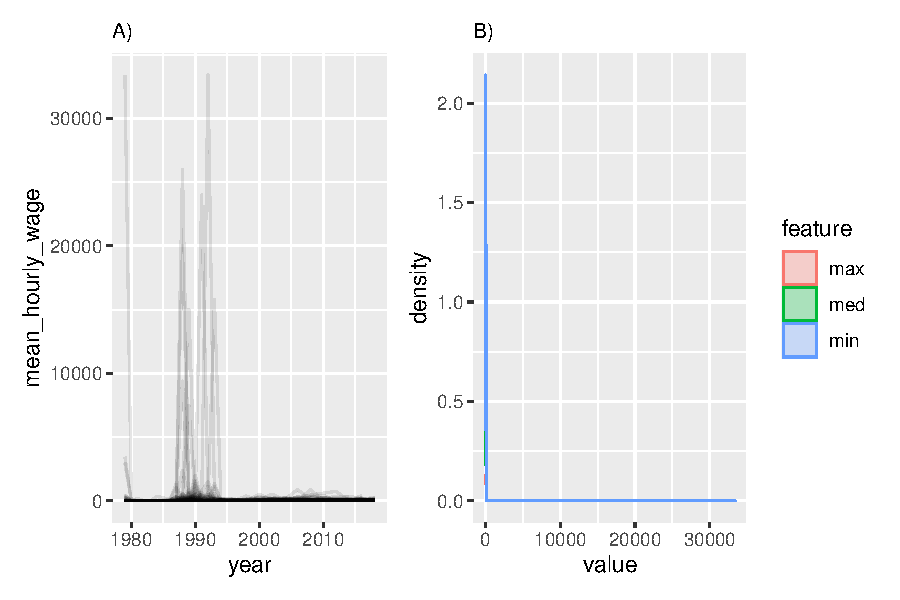
\includegraphics{figures/featureplot-1} \caption[Two plots showing the distribution of the mean hourly wage]{Two plots showing the distribution of the mean hourly wage. Plot A portrays the pattern of mean hourly wage of high school cohort from 1979 to 2018 of each ID in US Dollar; Plot B shows the distribution of their minimum, median, and maximum value. We can see that some IDs had an extremely high of wages and it made the distribution of the three features is extremely skewed.}\label{fig:featureplot}
\end{figure}
\end{Schunk}

The next step is that we explored the mean hourly wage data, in this
case, we only explored the wages data in \texttt{wages\_demog\_hs}.
Figure @ref(fig:featureplot) conveys that there is clearly a problem in
the mean hourly wage values. Figure \ref{fig:featureplot} A shows that
some observations had an exceptionally high figure of wages, even more
than US\$10,000 per hour. In Figure \ref{fig:featureplot} B, we barely
see any difference in the minimum, median, an maximum value of the wages
since the distribution is heavily skewed to the right. Additionally,
Table \ref{tab:summarytable} shows that the overall wages median of the
cohort is only 7.2, while the mean is 11.87. It indicates that the data
might contains a lot of extreme values.

\begin{Schunk}
\begin{table}

\caption{\label{tab:summarytable}Summary Statistics of Wages of High School Data}
\centering
\begin{tabular}[t]{l|r}
\hline
Statistics & Value\\
\hline
\rowcolor{gray!6}  Min. & 0.01000\\
\hline
1st Qu. & 4.50000\\
\hline
\rowcolor{gray!6}  Median & 7.20000\\
\hline
Mean & 11.86578\\
\hline
\rowcolor{gray!6}  3rd Qu. & 11.74000\\
\hline
Max. & 33400.00000\\
\hline
\end{tabular}
\end{table}

\end{Schunk}

In Figure \ref{fig:high-wages}, we plotted some respondents with a high
value of mean hourly wages. We filtered all of the IDs who earned more
than US\$ 500 per hour averagely. We found that most of these
respondents only experienced one point of extremely high wages. Thus, we
suspected that these high values are erroneous values resulted from a
data entry error.

\begin{Schunk}
\begin{figure}
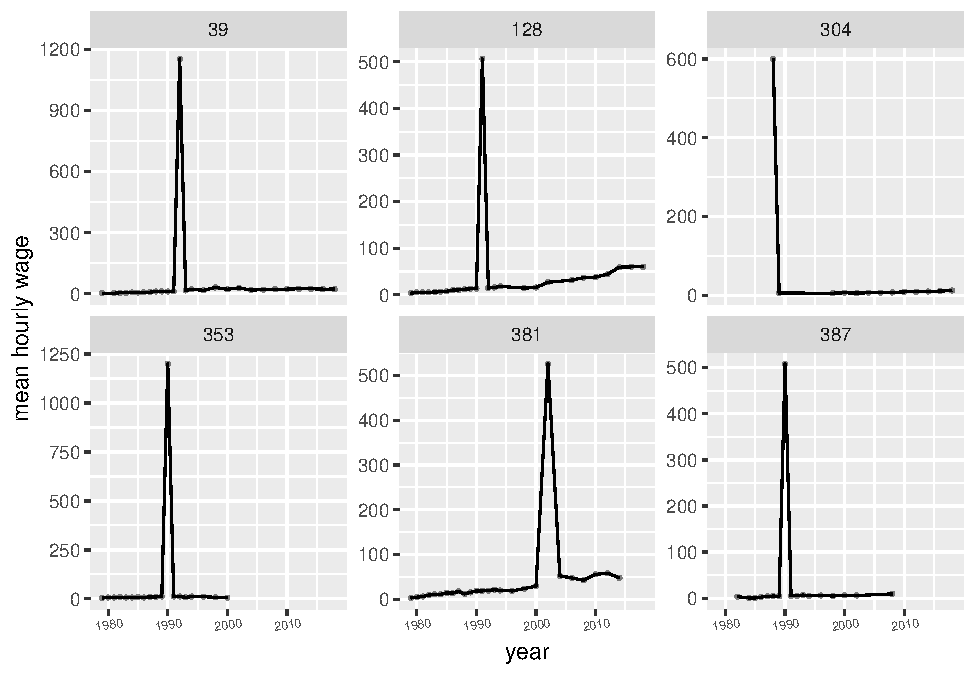
\includegraphics{figures/high-wages-1} \caption[Some observations with extremely high mean hourly wage]{Some observations with extremely high mean hourly wage. Most of the IDs only have one point of high wage.}\label{fig:high-wages}
\end{figure}
\end{Schunk}

Further, we took 36 samples randomly from the data and plotted it as is
seen in Figure \ref{fig:sampleplot}. It implies that not only that some
observations earned an extremely high figures of wages, but some also
had a reasonably fluctuate wages, for example the IDs in panel number 5,
7, and 11. The plot also implies that the samples had a different
pattern of mean hourly wages. Some had a flat wages for years but had a
sudden increase in a year than it went down again, while the other
experienced a upsurge in their wage, for instance the IDs in panel 9.

According to \citet{MichaelRPergamit2001DWTN}, one of the flaws of the
NLSY79 employment data is that since the NLSY79 collect the information
of the working hours since the last interview, it might be challenging
for the respondents to track the within-job hours changes that happens
between survey year, especially for the respondents with fluctuate
working hours or whose job is seasonal. It even has been more
challenging since 1994, where the respondents had to recall two years
period. This shortcoming might also contribute on the fluctuation of
one's wages data.

\begin{Schunk}
\begin{figure}
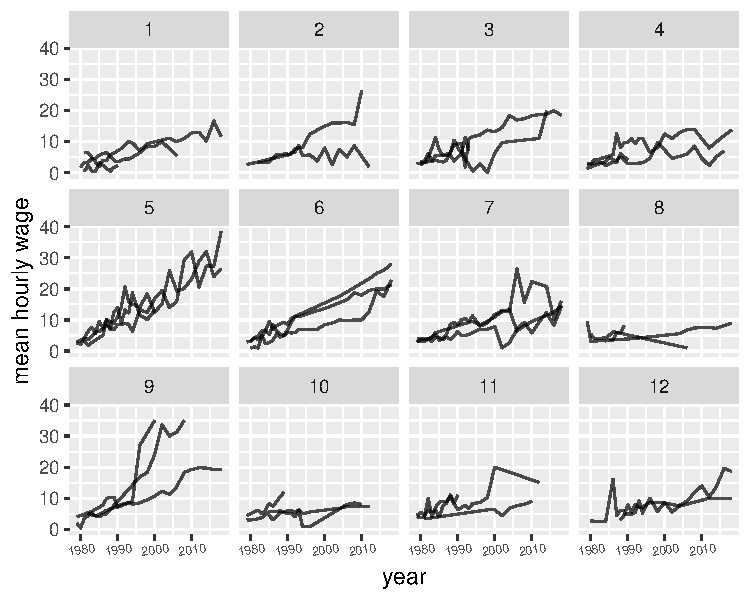
\includegraphics{figures/sampleplot-1} \caption[The mean hourly wages of some random samples are shown in twelve facets, three IDs per facet]{The mean hourly wages of some random samples are shown in twelve facets, three IDs per facet. It suggests that some IDs had a reasonably fluctuate wages.}\label{fig:sampleplot}
\end{figure}
\end{Schunk}

\hypertarget{replacing-extreme-values}{%
\subsubsection{Replacing extreme
values}\label{replacing-extreme-values}}

As it is seen from figure \ref{fig:sampleplot}, there are many spikes in
the mean hourly wage data. As part of the IDA, which is the model
formulation, we built a robust linear regression model to address this
issue. The notion of robust linear regression is to yield an estimation
that is robust to the influence of noise or contamination
\citep{KollerManuel2016rARP}. It also aims to detect the contamination
by weighting each observation based on how ``well-behave'' they are,
known as robustness weight. Observations with lower robustness weight
are suggested as an outliers by this method
\citep{KollerManuel2016rARP}.

In this paper, we built the model using the \texttt{rlm} function from
\texttt{MASS} package \citep{mass}. We set the
\texttt{mean\_hourly\_wage} and \texttt{year} as the dependent and
predictor respectively. Furthermore, we used M-Estimation with Huber
weighting where the observation with small residual get a weight of 1,
while the larger the residual, the smaller the weight (less than 1)
\citep{rlm}.

Since we worked with longitudinal data, we should built the model for
each ID, instead of the overall data. The robust mixed model is actually
the best model to be employed in this case. However, this method is too
computationally and memory expensive, especially for a large data set,
like the NLSY79 data. Thus, the model for each ID is built utilizing the
\texttt{nest} and \texttt{map} function from \texttt{tidyr}
\citep{tidyr} and \texttt{purrr} \citep{purrr} respectively.

The challenging part of detecting the anomaly using the robustness
weight is to determine the threshold of the weight where the
observations considered as outliers. Moreover, it should be noted that
not all the outliers is due to an error, instead it might be that one
had a reasonably increasing or decreasing wages. To, minimize the risk
of being mistakenly regard an outlier as an ``erronous outlier'', we
have simulated some threshold and study the behavior of the spikes in
each threshold. We found that 0.12 is the most reasonable value to be
the threshold to minimize the risk of that drawback because it still
capture the sensible spikes in the data. In other words, we kept
maintaining the natural variability of the wages while minimizing the
presence of anomalies because of the error in the data recording. After
deciding the threshold, we imputed the observations with weight less
than 0.2 wage with the models' predicted value. We then flagged those
observations in a new variable called \texttt{is\_pred},

\begin{Schunk}
\begin{Sinput}
# nest the data by id to build a robust linear model
by_id <- wages_demog_hs %>%
  dplyr::select(id, year, mean_hourly_wage) %>%
  group_by(id) %>%
  nest()

# build a robust linear model
id_rlm <- by_id %>%
  mutate(model = map(.x = data,
                     .f = function(x){
                       rlm(mean_hourly_wage ~ year, data = x)
                     }))
# extract the property of the regression model
id_aug <- id_rlm %>%
  mutate(augmented = map(model, broom::augment)) %>%
  unnest(augmented)

# extract the weight of each observation
id_w <- id_rlm %>%
  mutate(w = map(.x = model,
                 .f = function(x){
                   x$w
                 })) %>%
  unnest(w) %>%
  dplyr::select(w)

# bind the property of each observation with their weight
id_aug_w <- cbind(id_aug, id_w) %>%
  dplyr::select(`id...1`,
                year,
                mean_hourly_wage,
                .fitted,
                .resid,
                .hat,
                .sigma,
                w) %>%
  rename(id = `id...1`)

# if the weight < 1, the mean_hourly_wage is replaced by the model's fitted/predicted value.
# and add the flag whether the observation is predicted value or not.
# since the fitted value is sometimes <0, and wages value could never be negative,
# we keep the mean hourly wage value even its weight < 1.

wages_rlm_dat <- id_aug_w %>%
  mutate(wages_rlm = ifelse(w < 0.12  & .fitted >= 0, .fitted,
                            mean_hourly_wage)) %>%
  mutate(is_pred = ifelse(w < 0.12 & .fitted >= 0, TRUE,
                          FALSE)) %>%
  dplyr::select(id, year, wages_rlm, is_pred)

# join back the `wages_rlm_dat` to `wages_demog_hs`

wages_demog_hs <- left_join(wages_demog_hs, wages_rlm_dat, by = c("id", "year"))
\end{Sinput}
\end{Schunk}

Figure \ref{fig:comppict} A shows that after imputing the anomalies with
the models' predicted value, the highest wages value has decreased to be
around \$350. The spikes were still observed, but are not as extreme as
the original data set. In Figure \ref{fig:comppict} B), we plotted the
three features of mean hourly wages, namely the minimum, median, an
maximum value, transformed to log scale. The plot implies that the
skewness are slightly negative. We also see that the three features are
overlapped each other. It indicates that some ID's minimum wage are
higher than some ID's maximum wage.

Furthermore, Figure \ref{fig:compare} implies that after the treatment,
the fluctuation can still be observed in the data and only the large
spikes, which are considered as ``erronous outliers'', are eliminated
from the data. Hence, the model results a data set with the reasonable
degree of fluctuation.

\begin{Schunk}
\begin{figure}
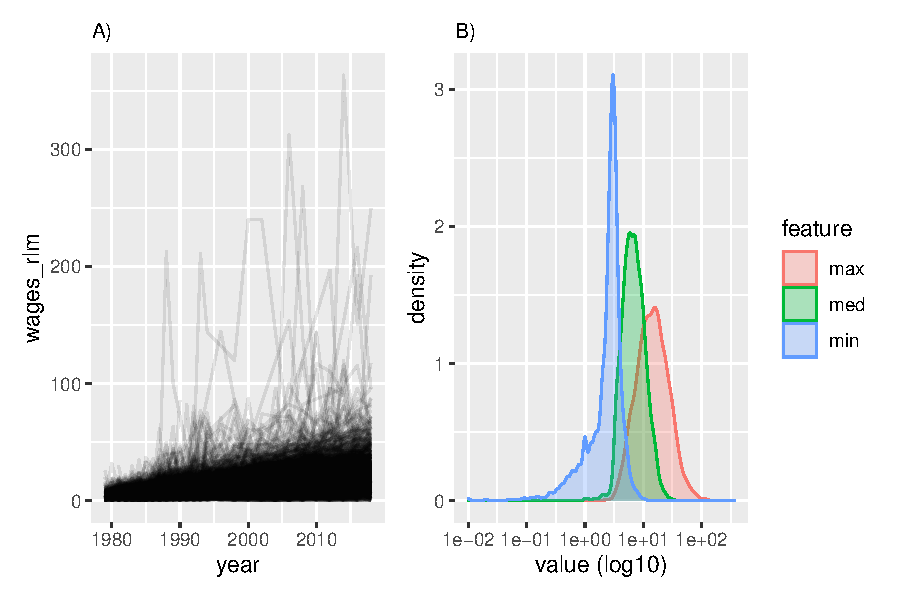
\includegraphics{figures/comppict-1} \caption[The distribution of the mean hourly wage after treating the extreme values]{The distribution of the mean hourly wage after treating the extreme values. Plot A portrays the pattern of mean hourly wage of high school cohort from 1979 to 2018 of each ID in US Dollar; Plot B shows the distribution of their minimum, median, and maximum value transformed to log10 scale. We can see that some observations still had reasonbaly higher wages than the others. Also, some IDs' have a minimum wages that is higher than others' maximum wages.}\label{fig:comppict}
\end{figure}
\end{Schunk}

\begin{Schunk}
\begin{figure}
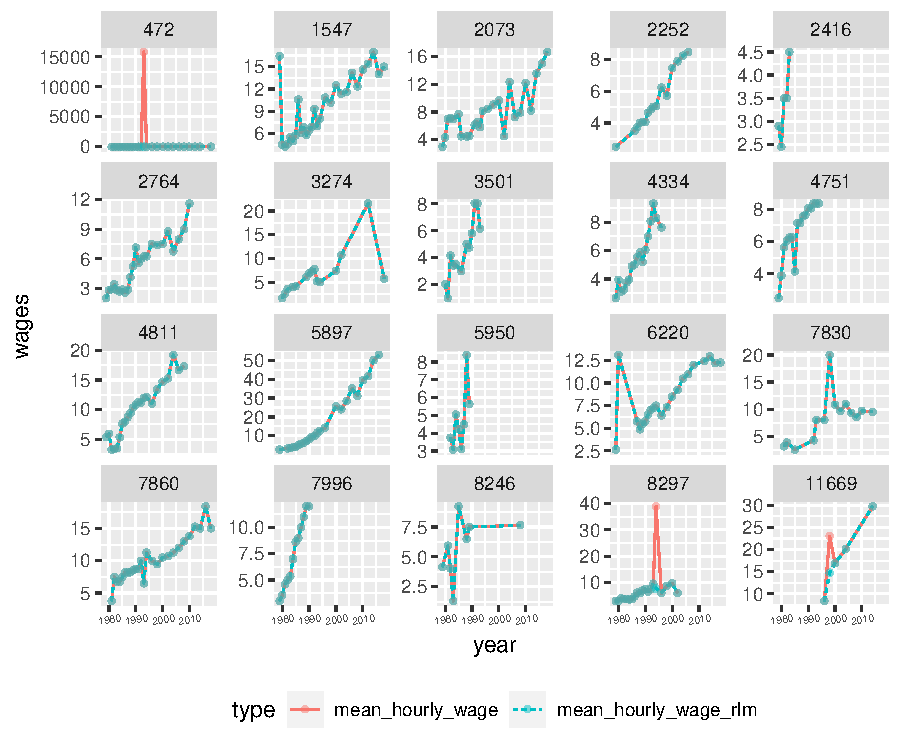
\includegraphics{figures/compare-1} \caption[Comparison between the original and the treated mean hourly wage]{Comparison between the original and the treated mean hourly wage. The orange line portray the original value of mean hourly wage, while the turquoise line display the mean hourly wages value after the extreme values imputed with the robust linear model's prediction value. We can see that some extreme spikes has been reduced by the model.}\label{fig:compare}
\end{figure}
\end{Schunk}

Finally, we saved the imputed data and set the appropriate data type for
the variables. As our target data is the mean hourly wage of the
high-school dropouts, we then subset the high-school graduate data set
to be only having the male-high school dropout data. We also saved the
NLSY79 cohort's demographic information in a separate dataset. We then
make these three data sets and its processing documentation to be
publicly available through an R data container package called
\texttt{yowie}. The complete flow from the raw data to these data set is
displayed in Figure \ref(fig:flowchart).

\begin{Schunk}
\begin{Sinput}
# select out the old value of mean hourly wage and change it with the wages_rlm value
wages_demog_hs <- wages_demog_hs %>%
  dplyr::select(-mean_hourly_wage) %>%
  rename(mean_hourly_wage = wages_rlm)

# rename and select the wages in tidy
wages_hs2020 <- wages_demog_hs %>%
  dplyr::select(id, year, mean_hourly_wage, age_1979, gender, race, hgc, hgc_i, yr_hgc,
                number_of_jobs, total_hours, is_wm, is_pred) %>%
  mutate(hgc = as.factor(hgc),
         year = as.integer(year),
         age_1979 = as.integer(age_1979),
         yr_hgc = as.integer(yr_hgc),
         number_of_jobs = as.integer(number_of_jobs))

# Create a data set for demographic variables
demographic_nlsy79 <- full_demographics %>%
  mutate(age_1979 = 1979 - (dob_year + 1900)) %>%
  dplyr::select(id,
         age_1979,
         gender,
         race,
         hgc,
         hgc_i,
         yr_hgc) %>%
  mutate(age_1979 = as.integer(age_1979),
         hgc = as.factor(hgc),
         yr_hgc = as.integer(yr_hgc))

# Create a data set for the high school dropouts cohort
wages_hs_dropout <- wages_hs2020 %>%
  mutate(dob = 1979 - age_1979,
         age_hgc = yr_hgc - dob) %>%
  filter((hgc %in% c("9TH GRADE",
                     "10TH GRADE",
                     "11TH GRADE")) |
          (hgc == "12TH GRADE" &
              age_hgc > 19)) %>%
  filter(age_1979 <= 17,
         gender == "MALE") %>%
  dplyr::select(-dob,
         -age_hgc)
\end{Sinput}
\end{Schunk}

\begin{Schunk}
\begin{figure}

\includegraphics{figures/flowchart-1} \caption[The stages of data filtering from the raw data to get three datasets that are contained in an R package called yowie, n means the number of ID, while n_obs means the number of observations]{The stages of data filtering from the raw data to get three datasets that are contained in an R package called yowie, n means the number of ID, while n_obs means the number of observations.}\label{fig:flowchart}
\end{figure}
\end{Schunk}

\hypertarget{exploratory-data-analysis}{%
\section{Exploratory Data Analysis}\label{exploratory-data-analysis}}

In this part, we gave some examples of how the data might be used for
data analysis in text book. We used \texttt{brolgar} \citep{brolgar} to
perform exploratory data analysis. The first example is that we observed
relationship between wages and education in terms of how the wages
increase year by year. Using \texttt{key\_slope} function in
\texttt{brolgar}, we performed a liner regression with mean hourly wage
as response variable and year as predictor and extracted the regression
slope of each ID and plotted it according to highest grade completed.

We found in Figure \ref{fig:wages-slope} that the higher the education
completed does not necessarily increase the wages more from year to
year. We can see that people who completed 4th grade happen to have
relatively the same median of slope as people who completed 11th grade,
even though it is probably because some respondents in this group had an
extremely high mean hourly wages. Moreover, the annual increasing wages
of people who completed 6th grade to 11th grade are relatively same.
People who completed 12th grade tend to have higher slope of year
compared to the other groups. Some outliers are also spotted in this
group. Additionally, we can see that some respondents have a negative
slope, meaning that their wages tend to decrease over the year.

\begin{Schunk}
\begin{figure}
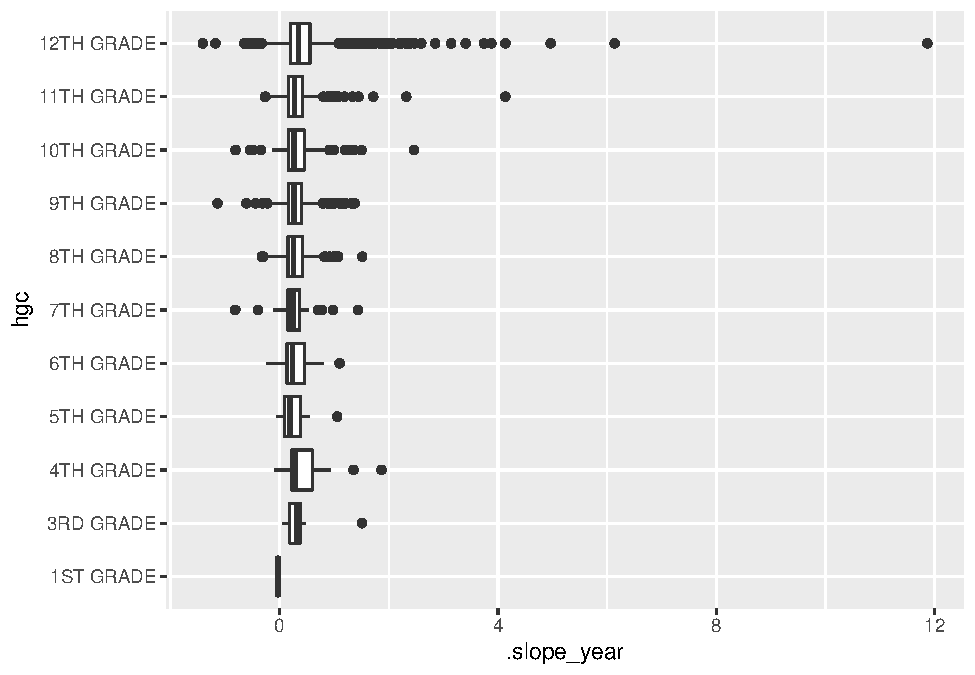
\includegraphics{figures/wages-slope-1} \caption[Regression slope of mean hourly wage regression by highest grade completed]{Regression slope of mean hourly wage regression by highest grade completed. The regression model has mean hourly wage as response variable and year as predictor. Respondents who completed 12th grade has the highest median of slope.}\label{fig:wages-slope}
\end{figure}
\end{Schunk}

In the second example, we examined the pattern of mean hourly wage
corresponding to different groups of gender and race. We took 240
samples of female and male equally and spread it into twelve facets as
is seen in Figure \ref{fig:gender-plot} using \texttt{facet\_strata}
function from \texttt{brolgar} \citep{brolgar}. We learn that the mean
hourly wage of female and male fluctuated over the years. In some
facets, for example in facet 4, 5, and 10, males tend to earn more wages
than females. This finding is also shown in Figure \ref{fig:gender-se}
where we plotted the median wage of males and females against the year.
We learn that males had a higher mean of mean hourly wage over the
period of survey than females. Unfortunately, the gap between them tend
to be wider from time to time.

\begin{Schunk}
\begin{figure}
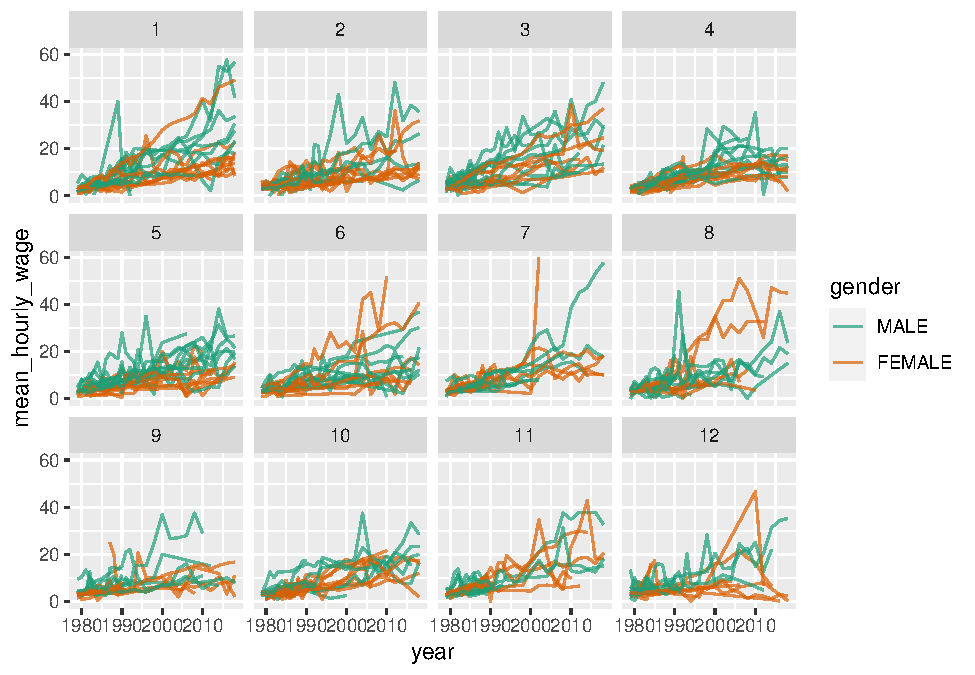
\includegraphics{figures/gender-plot-1} \caption[The pattern of mean hourly wages overtime displayed in 12 facets coloured by gender]{The pattern of mean hourly wages overtime displayed in 12 facets coloured by gender. The respondents belong to high school cohort are randomly sampled. We learn that both male and female respondents had a fluctuate mean hourly wage over the year.}\label{fig:gender-plot}
\end{figure}
\end{Schunk}

\begin{Schunk}
\begin{figure}
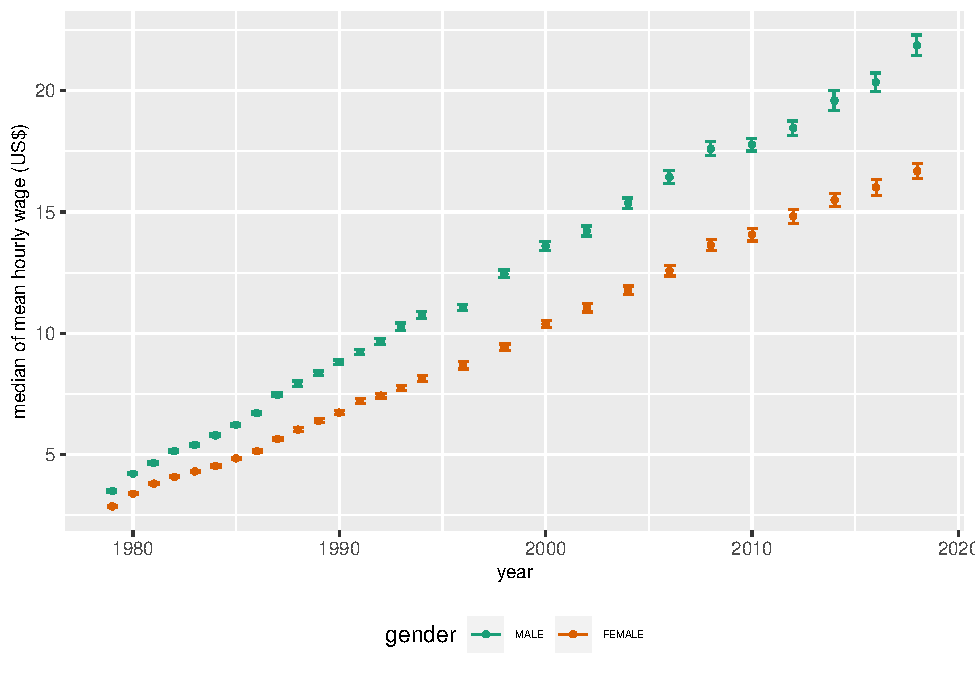
\includegraphics{figures/gender-se-1} \caption[The yearly mean of mean hourly wage by gender along with its standard error]{The yearly mean of mean hourly wage by gender along with its standard error. Males generally earn more wages than females. The error interval tend to be wider over the years.}\label{fig:gender-se}
\end{figure}
\end{Schunk}

For the final example, we show the example of modeling the longitudinal
data using Generelized Additive Model (GAM) with \texttt{mgcv} package
\citep{mgcv} for each ID. We fit a more flexible model to fit in to the
data since the relationship between mean hourly wage and year is not
linear due to the spikes. Since this approach is computationally
expensive, we only show the model in a little fraction of the data. We
sample 1 percent of the total respondents using
\texttt{brolgar\textquotesingle{}s} \texttt{sample\_frac\_keys}
function. Further, we plotted the some sample of the fitted model in
Figure @ref\{fig:gam-plot\}. We learn that the model flexible enough to
deal with the fluctuation in the data. Moreover, model with small spikes
tend to be linearly fitted.

\begin{Schunk}
\begin{figure}
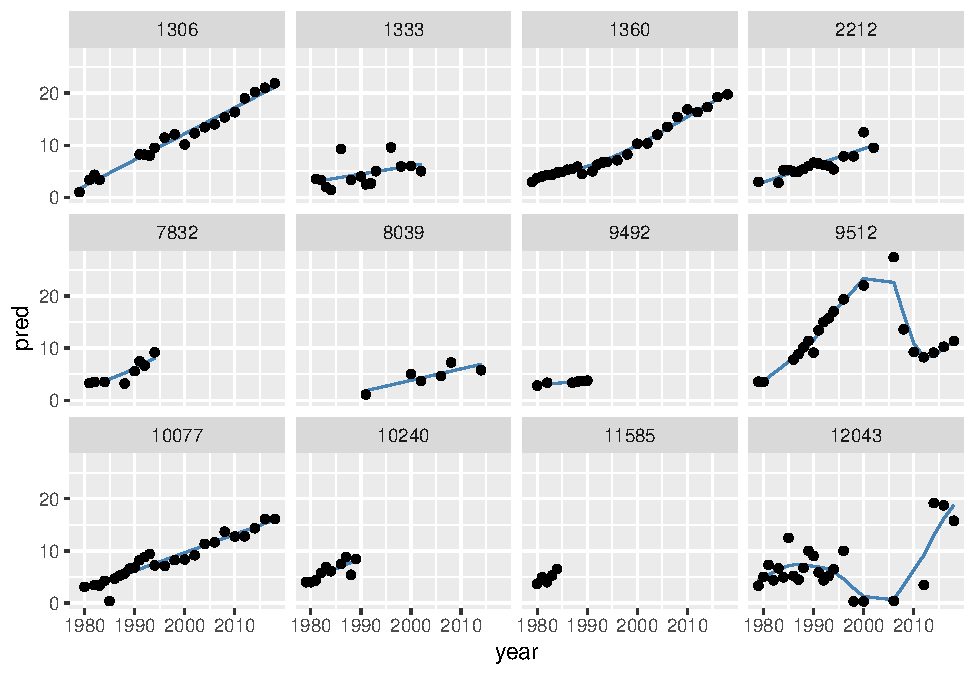
\includegraphics{figures/gam-plot-1} \caption[Exploration of wages data by fitting a GAM]{Exploration of wages data by fitting a GAM. The fitted model displayed by blue line. The fitted line shows that the model flexible enough to follow the pattern of the data.}\label{fig:gam-plot}
\end{figure}
\end{Schunk}

\hypertarget{summary}{%
\section{Summary}\label{summary}}

This paper has performed a set of stages to make an open data suitable
for a text book data or to make it ready for research. In the first
stage, we showed the steps that are performed to get the data from the
NLSY79 database. Since the data format is untidy, we showed how the data
has been tidied. After that, we conducted an initial data analysis to
investigate and screen the quality of the data. Using robust linear
regression model, we found and fixed the anomalous observations in the
data set with its predicted values. We also performed an example of
exploratory data analysis using the cleaned data set.

This paper also has demonstrated the documentation of data cleaning by
providing all of the codes in performing data tidying and initial data
analysis. Thus, this paper provided an opportunity to continuously
refresh the text book data whenever the updated data is published in the
NLSY79 database. This could be done by following the documentation of
the code that is provided in this paper.

Moreover, the documentation also includes the process of how did we
generate the robustness weight and how did we decide the threshold of
anomalous observations. It is also documented along with the flag of
whether an observation is imputed value or not. Accordingly, if somebody
wish to make another decision, it can be done by making a small changes
in the code provided. Further, this paper is also supplemented by a
\texttt{shiny} \citep{shiny} app as a simulation tool to customize the
weight threshold.

Finally, this paper implies that data providers should design the
database that is able to produce tidy data sets. A data provider should
also check for data anomalies prior the data publishing or at least
provides a set of rules or threshold value, for example, in this case is
the threshold of reasonable wages. This will greatly support the data
users to carry out further validation and set the same understanding of
which data are considered as outliers. Moreover, providing validation
rules would facilitate the usage of any establish data validation tool,
such as \texttt{validate} \citep{validate} package. In this case, we
cannot use this handy validation package due to the absence of
validation rules.

\hypertarget{acknowledgements}{%
\section{Acknowledgements}\label{acknowledgements}}

We would like to thank Aarathy Babu for the insight and discussion
during the writing of this paper.

The entire analysis is conducted using \texttt{R} \citep{R} in
\texttt{rstudio} using these packages: \texttt{tidyverse}
\citep{tidyverse}, \texttt{ggplot2} \citep{ggplot2}, \texttt{dplyr}
\citep{dplyr}, \texttt{readr} \citep{readr}, \texttt{tidyr}
\citep{tidyr}, \texttt{stringr} \citep{stringr}, \texttt{purrr}
\citep{purrr}, \texttt{broom} \citep{broom}, \texttt{blorgar}
\citep{brolgar}, \texttt{patchwork} \citep{patchwork},
\texttt{kableExtra} \citep{kableExtra}, \texttt{MASS} \citep{mass},
\texttt{janitor} \citep{janitor}, \texttt{DiagrammeR}
\citep{DiagrammeR}, \texttt{rsvg} \citep{rsvg}, \texttt{webshot}
\citep{webshot}, \texttt{mgcv} \citep{mgcv}, \texttt{tsibble}
\citep{tsibble}, and \texttt{modelr} \citep{modelr}. The paper are
generated using \texttt{knitr} \citep{knitr}, \texttt{rmarkdown}
\citep{rmarkdown}, and \texttt{rticles} \citep{rticles}.

\hypertarget{supplementary-materials}{%
\section{Supplementary Materials}\label{supplementary-materials}}

\begin{itemize}
\item
  \textbf{Codes} : R script to reproduce data tidying and cleaning are
  available in this
  \href{https://github.com/numbats/yowie/blob/master/data-raw/data_preprocessing.R}{Github
  Repository}.
\item
  \textbf{R Package \texttt{yowie}}:\texttt{yowie} is a data container R
  package that contains 3 datasets, namely the high school mean hourly
  wage data, high school dropouts mean hourly wage data, and demographic
  data of the NLSY79 cohort. This package could be accessed
  \href{https://github.com/numbats/yowie}{here}.
\item
  \textbf{shiny app}: An web interactive \texttt{shiny} app to run a
  simulation to customize the weight threshold. This app could be
  accessed
  \href{https://github.com/numbats/summer-wages-refresh/tree/main/app}{here}.
\end{itemize}

\bibliography{references.bib}

